\documentclass[tikz,fontsize=8pt,border=0pt]{standalone}
\usepackage{fourier}
\usetikzlibrary{arrows.meta}
\usetikzlibrary{calc}
\tikzset{>=latex}
\definecolor{bookblue}{RGB}{0,173,239}
\definecolor{bookpink}{RGB}{236,0,140}
\definecolor{bookgreen}{RGB}{50,200,0}
\definecolor{bookbluearea}{RGB}{204,239,252}
\tikzstyle{blueline}=[draw=bookblue,line width=0.2mm]
\tikzstyle{pinkline}=[draw=bookpink,line width=0.2mm]
\tikzstyle{greenline}=[draw=bookgreen,line width=0.2mm]
\tikzstyle{blackline}=[draw=black,line width=0.2mm]
\tikzstyle{bluearea}=[fill=bookbluearea]

\usepackage{scrextend}
\changefontsizes[8pt]{8pt}
\usetikzlibrary{decorations.pathreplacing}
\begin{document}
  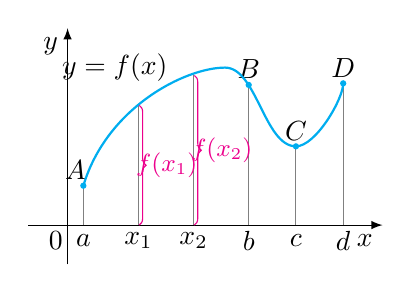
\begin{tikzpicture}
  %\useasboundingbox (-0.01,-1.51) rectangle (4.01,2.51);
  \node at (-0.15,-0.2) {0};
  \node at (0.2,-0.2) {$a$};
  \node at (0.9,-0.2) {$x_1$};
  \node at (1.6,-0.2) {$x_2$};
  \node at (2.3,-0.2) {$b$};
  \node at (2.9,-0.2) {$c$};
  \node at (3.5,-0.2) {$d$};
  \draw[->] (-0.5,0) -- (4,0) node[below left] {$x$};
  \draw[->] (0,-0.5) -- (0,2.5) node[below left] {$y$};
  
  
  \draw[gray] (0.2,0) -- (0.2,0.5);
  \fill[bookblue] (0.2,0.5) circle (0.4mm) node[black,yshift=2mm,xshift=-1mm] {$A$};

  \draw[gray] (0.9,0) -- (0.9,1.53);
  \draw[gray] (1.6,0) -- (1.6,1.935);
  
  \draw[gray] (2.3,0) -- (2.3,1.78);
  \fill[bookblue] (2.3,1.78) circle 
  (0.4mm)node[black,yshift=2mm,xshift=-0mm] {$B$};
  
  \draw[gray] (2.9,0) -- (2.9,1);
  \fill[bookblue] (2.9,1) circle (0.4mm)node[black,yshift=2mm,xshift=-0mm] {$C$};
  
  \draw[gray] (3.5,0) -- (3.5,1.8);
  \fill[bookblue] (3.5,1.8) circle (0.4mm)node[black,yshift=2mm,xshift=-0mm] {$D$};
  \draw[bookblue, thick]
    (0.2,0.5) 
    .. controls (0.5,1.5) and (1.5,2) .. 
    (2,2) 
    .. controls (2.4,2) and (2.5,1) .. 
    (2.9,1)
    .. controls (3.15,1) and (3.5,1.6) .. 
    (3.5,1.8);
  \node at (0.6,2) {$y=f(x)$};
  \draw [bookpink,decorate,decoration={brace,mirror},xshift=-4pt,yshift=0pt]
  (1.05,0) -- (1.05,1.52) node [bookpink,midway,xshift=0.35cm] 
  {\small $f(x_1)$};
  \draw [bookpink,decorate,decoration={brace,mirror},xshift=-4pt,yshift=0pt]
  (1.75,0) -- (1.75,1.9) node [bookpink,midway,xshift=0.35cm] 
  {\small $f(x_2)$};
  
  %\draw [dashed, line width=0.2mm] (0.68,0) -- (0.68,0.8);
  %\draw [dashed, line width=0.2mm] (1.78,0) -- (1.78,1.38);
  
  %\draw[blackline,domain=-1.1:0.5] plot (\x+1.5,{-(\x)^2+1.5});
  %\draw[pinkline] (0.256,0.15) -- (1.356,1.91);
  %\node at (0.05,0.83) {$P(a,f(a))$};
  %\node at (1.2,2) {$t$};
  %\node at (2.1,1.7) {$Q(x, f(x))$};
  %\draw [decorate,decoration={brace,mirror},xshift=-4pt,yshift=0pt]
  %(0.85,0.78) -- (1.88,0.78) node [black,midway,yshift=-0.3cm] 
  %{\footnotesize $x-a$};
  %\draw [decorate,decoration={brace,mirror},xshift=-4pt,yshift=0pt]
  %(1.95,0.83) -- (1.95,1.38) node [black,midway,xshift=0.65cm] 
  %{\footnotesize $f(x)-f(a)$};
  %\draw[greenline] (0.7,0.83) -- (1.78,0.83);
  %\draw[greenline] (1.78,0.83) -- (1.78,1.43);
  %\draw[blueline]  (-0.3,0.3) -- (2.3,1.7);
  %\fill (0.68,0.83) circle (0.4mm);
  %\fill (1.78,1.42) circle (0.4mm);
  %\node at (0.65,-0.15) {$a$};
  %\node at (1.75,-0.15) {$x$};
  \end{tikzpicture}
\end{document}